\documentclass[12pt,letterpaper]{article}

\newenvironment{proof}{\noindent{\bf Proof:}}{\qed\bigskip}

\newtheorem{theorem}{Theorem}
\newtheorem{corollary}{Corollary}
\newtheorem{lemma}{Lemma} 
\newtheorem{claim}{Claim}
\newtheorem{fact}{Fact}
\newtheorem{definition}{Definition}
\newtheorem{assumption}{Assumption}
\newtheorem{observation}{Observation}
\newtheorem{example}{Example}
\newcommand{\qed}{\rule{7pt}{7pt}}

\newcommand{\assignment}[4]{
\thispagestyle{plain} 
\newpage
\setcounter{page}{1}
\noindent
\begin{center}
\framebox{ \vbox{ \hbox to 6.28in
{\bf CS446: Machine Learning \hfill #1}
\vspace{4mm}
\hbox to 6.28in
{\hspace{2.5in}\large\mbox{Problem Set #2}}
\vspace{4mm}
\hbox to 6.28in
{{\it Handed Out: #3 \hfill Due: #4}}
}}
\end{center}
}

\newcommand{\solution}[4]{
\thispagestyle{plain} 
\newpage
\setcounter{page}{1}
\noindent
\begin{center}
\framebox{ \vbox{ \hbox to 6.28in
{\bf CS446: Machine Learning \hfill #4}
\vspace{4mm}
\hbox to 6.28in
{\hspace{2.5in}\large\mbox{Problem Set #3}}
\vspace{4mm}
\hbox to 6.28in
{#1 \hfill {\it Handed In: #2}}
}}
\end{center}
\markright{#1}
}

\newenvironment{algorithm}
{\begin{center}
\begin{tabular}{|l|}
\hline
\begin{minipage}{1in}
\begin{tabbing}
\quad\=\qquad\=\qquad\=\qquad\=\qquad\=\qquad\=\qquad\=\kill}
{\end{tabbing}
\end{minipage} \\
\hline
\end{tabular}
\end{center}}

\def\Comment#1{\textsf{\textsl{$\langle\!\langle$#1\/$\rangle\!\rangle$}}}



\usepackage{graphicx,amssymb,amsmath, listings}
\lstset{language = Matlab}
\lstset{breaklines}
\lstset{extendedchars=false}

\oddsidemargin 0in
\evensidemargin 0in
\textwidth 6.5in
\topmargin -0.5in
\textheight 9.0in
\begin{document}

\solution{Jifu Zhao}{10/22/2015}{4}{Fall 2015}
% Fill in the above, for example, as follows:
% \solution{Joe Smith}{\today}{1}{Fall 2012}

\pagestyle{myheadings}  % Leave this command alone

\begin{enumerate}
\item {\bf Answer to problem 1}
\begin{enumerate}
\item[(a)\\]
For the concept space of triangles in the place, the VC dimension are {\bf 7}.\\

{\bf Proof:} Now, suppose that our points are distributed in a convex hull (like a circle). for 1 to 6 points, it is easy to find that the triangles can successfully shattered them arbitrarily. When, there is 7 points, as shown in Figure 1. It is easy to prove that we can separate any 1, 2, 3, 4, 5, 6 or 7 points using one triangle. So, the VC dimension will at least be 7. But when there is 8 points, as shown in the right picture, when the label is +, -, +, -, +, -, +, -, it is not possible to separate one negative point from other 4 positive points.
\begin{figure}[h!]

  \centering
    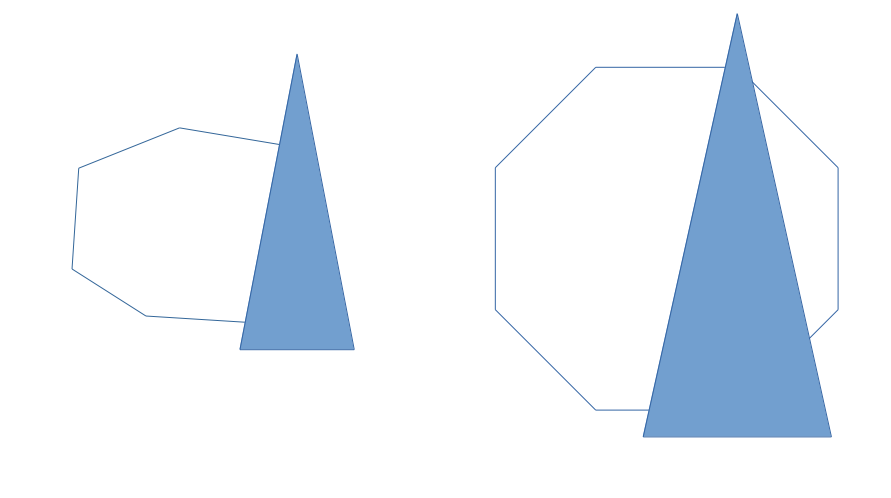
\includegraphics[width=0.7\textwidth]{7.png}
      \caption{7 and 8 points.}
\end{figure}

So, the VC dimension of triangles will be 7.\\

\item[(b)\\]
For the concept space of the union of k disjoint intervals in a real line, the VC dimension are {\bf 2k}.\\

{\bf Proof:} First, let's prove that there will be at least 2k points that can be shattered. Now, consider only two points, the labels can be ++, +-, -+ and --. So, one interval can separate two points. But when there is 3 points, if the labels is +-+, then we cannot separate it. So, for one interval, the VC dimension is 2. This conclusion can be easily broaden to multiple intervals. When there is k distinct intervals, it is reasonable to conclude that the VC dimension should be at least 2k.\\

Now, let's find its upper bound. When there is 2k+1 points in a real line. Assume that their label is +-+-......+-+. There is 2k+1 points. So, for every points that is labelled +, we need an interval [a, b] to include the point. So, for the first k positive points, we need k intervals. But there is one last positive point that cannot be included by any interval. So, the VC dimension for k disjoint intervals in a real line will be less that 2k+1.\\

So, to conclude, the VC dimension for k disjoint intervals in a real line will be {\bf 2k}.\\

\end{enumerate}

\item {\bf Answer to problem 2}
\begin{enumerate}
\item[(a)]
Suppose that $c = <(c_1, b_1), ... (c_l, b_l), b>$, so, c could be $b_1, b_2, ..., b_l, b$. As a corresponding, $\neg c$ should be: $\neg b_1, \neg b_2, ..., \neg b_l, \neg b$. So, we can easily write $c$ as:
\begin{center}
$\neg c = <(c_1, \neg b_1), ... (c_l, \neg b_l), \neg b>$
\end{center}
So, if a concept c can be represented as a k-decision list, so can its complement, $\neg c$.\\
\item[(b)]

Let c denotes conjunctive clause containing at most k literals, and let d denotes disjunctive clause containing at most k literals. So, k-CNF and k-DNF can be written as:
\begin{center}
$ k-CNF = d_1 \wedge d_2 \wedge d_3...\wedge d_{n-1} \wedge d_n $\\
$ k-DNF = c_1 \vee c_2 \vee c_3...\vee c_{n-1} \vee c_n $
\end{center}

\begin{enumerate}
\item[1) ] First, let's consider k-DNF. if $ k-DNF = c_1 \vee c_2 \vee c_3...\vee c_{n-1} \vee c_n $, then, according to the definition of k-decision list, we can write k-DNF as the following functions:
\begin{center}
$f_{DNF} = <(c_1, 1), (c_2, 1), ... (c_n, 1), 0>$\\
\end{center}
It is clear that $f_{DNF} = k-DNF$.\\

So, we have proved that k-DNF can be written as k-decision list, so $$k\textrm{-DNF} \subseteq k\textrm{-DL}$$

\item[2) ] Now, let's consider k-CNF. According to the relationship between k-DNF and k-CNF, any k-CNF can be written as: 
$$k-CNF = d_1 \wedge d_2 \wedge d_3...\wedge d_{n-1} \wedge d_n$$
then we can written it as:
$$\neg k-CNF = \neg d_1 \vee \neg d_2 \vee \neg d_3... \vee  \neg d_{n-1} \vee \neg d_n \equiv k-DNF$$
And since that 
$$k\textrm{-DNF} \subseteq k\textrm{-DL}$$
So, $$\neg k\textrm{-CNF} \subseteq k\textrm{-DL}$$
Also, according to {\bf a}, $$\neg (\neg k\textrm{-CNF}) \subseteq k\textrm{-DL}$$
which means that $$k\textrm{-CNF} \subseteq k\textrm{-DL}$$
So, we proved that $$k\textrm{-CNF} \subseteq k\textrm{-DL}$$
\end{enumerate}

So, according to 1) and 2), we can conclude that:
$$k\textrm{-DNF} \cup k\textrm{-CNF} \subseteq k\textrm{-DL}$$

\item[(c)]

First, we need to list all the possible conjunction of at most k literals over $x_1, x_2, ... x_n$, which is a set named $Con_k$. The algorithm is as follows:\\
\rule{14cm}{0.4pt}
\begin{enumerate}
\item[1, ] Start with an empty decision list.
\item[2, ] For every conjunction $c_i$ in $Con_k$, selecting the data from S where $c_i(x) = 1$, which is a set named Pi. Compare $c_i$ with the data $L(x) = b$ from Pi. If $c_i$ is consistent with all the results from Pi, then stop, remember $c_i$ and its value in ($c_i$, b). If not consistent, move to $c_{i+1}$.
\item[3, ] Add ($c_i$, b) to the decision list. and remove the sample data in Pi from S. Using the new S for next step.
\item[4, ] If S is empty, quit. Else, return to step 2.
\end{enumerate}
\rule{14cm}{0.4pt}

{\bf Proof: }\\
The above algorithm is based on the condition that our sample data is consistent with at least one decision list. In this algorithm, when the S is empty, which means that we have successfully find all the conjunctions with all the data from S, the algorithm will stop. This means that we have successfully construct a k-decision list.\\

The algorithm will must stop. The reason is simple, the data is consistent with at least one k-decision list. In this algorithm, we have considered all the possible conjunctions, so, we will surely find the conjunctions that is consistent with every step.\\

Now, consider the correctness of the algorithm. Let's consider one example $L(x_i) = b_i$. Suppose that this item is removed from old S in the $N_{th}$ step. This mean that in the previous $(N-1)_{th}$ steps, there is no conjunction that is consistent with $L(x_i) = b_i$, and in the $N_{th}$ step, we find the conjunction that is consistent with $L(x_i) = b_i$, so we will build the new decision list. As this algorithm goes, we can make sure that for all sample data, we will assign them with the correct label(b) through our algorithm. So, our decision list will always be consistent will all the sample data.\\

One thing needed to be mentioned it that: the decision list can not be the same with the original decision list. It will absolutely be consistent with the sample data, but can be different from the original list.\\

\item[(d)]

For any constant $k \geq 1$, the size of possible conjunctions should be: $O(n^k)$. So, $$|C_k| = O(n^k).$$
As a result, now we consider the extreme situation, the maximum size of the hypothesis space $|H|$ will be: $$|H| = 2^{|C_k|} \cdot |C_k|! \cdot 2^{|C_k|} = 2^{2|C_k|} \cdot |C_k|!$$
So, according to the Occam's Razor, 
$$m > 1/\varepsilon (ln(|H|) + ln(1/\delta))$$
Now we only need to calculate $ln(|H|)$, where
$$ln(|H|) = 2|C_k|ln2 + ln(|C_k|!) = O(2|n^k|ln2 + ln(|n^k|!) = O(n^k)$$

So, its complexity will be the polynomial in n. So, we can say that {\bf the class of k-decision lists is efficiently PAC-learnable}.\\
\end{enumerate}

\item {\bf Answer to problem 3}
\begin{enumerate}
\item[(a)]
The kernel: $K(x, z) = \sum_{c \in C} c({\bf x}) c({\bf z})$, now let's consider the case where each term of the DNF is exactly of k literal. So, when calculate  $\sum_{c \in C} c({\bf x}) c({\bf z})$, we in fact are going to find all the k literals that is the same in both {\bf x} and {\bf z}. So, $\sum_{c \in C} c({\bf x}) c({\bf z}) = {same({\bf x},{\bf z}) \choose k}$. This is true only when we consider the exact k literals. When we are going to consider 1 to k literals, we only need to calculate the same equation for all possible literal numbers. So, we can get: $$K(x, z) = \sum_{i = 1}^{k}{same({\bf x},{\bf z}) \choose i}.$$ In this way, we only need to compare every item in both {\bf x} and {\bf z}, then choose i = 1 to k from them. This calculation is much easier, and its complexity should be {\bf polynomial in n}.\\

\item[(b)]

In the previous Perceptron method, we use $$f({\bf x}) = sgn({\bf w \cdot x} + \theta)$$
Now, with kernel $K(x, z)$, we can use Perceptron based on the kernel. We now use $$f({\bf x}) = \sum_{i = 1}^n (\alpha_j K({\bf x_i} \cdot {\bf x_j}))$$ The algorithm are shown below:
\begin{algorithm}
1, Initiate parameters to be 0: $\alpha_i = 0, i = 1 ... n$. \\

2, Calculate $temp = y_j \sum_{i = 1}^n (\alpha_i K({\bf x_i} \cdot {\bf x_j}))$.\\\

\qquad \qquad if $temp < 0$, add 1 to $\alpha_j$,  $\alpha_j = \alpha_j + 1$.\\

3, Repeat 2 until converge.\\

4, got $\alpha_j, j = 1, 2, 3 ...... n $\\

\end{algorithm}

\item[(c)]
Through the kernel, we have increased the number of features from $n$ to $2^kC(n, k) <= 2^kn^k$. So, the mistakes will definitely increase.\\

Using Novikoff's theorem, we can find that the mistake bound of the kernel Perciptron algorithm will be $2^k$.\\

\end{enumerate}

\end{enumerate}

\end{document}

